\section{Questão 1}
Uma nova carga deseja se instalar no sistema de potência cujo diagrama unifilar é mostrado na Figura 1. Os dados do sistema são mostrados nas Tabelas I e II.

\begin{figure}[h]
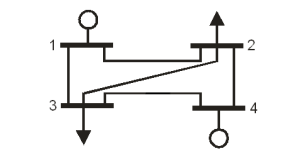
\includegraphics{fig1}
\centering
\caption{Diagrama Unifilar do Sistema}
\label{fig:fig1}
\end{figure}

\begin{figure}[h]
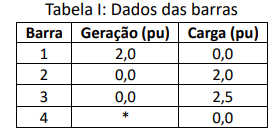
\includegraphics{tab1}
\centering
\end{figure}


*a barra 4 funciona como referência angular do sistema e possui capacidade máxima de 5,0 pu\\

\begin{figure}[h]
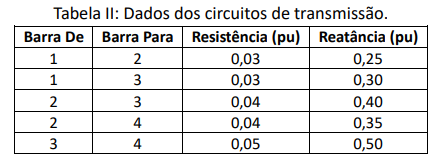
\includegraphics{tab2}
\centering
\end{figure}

A nova carga de 1,5 pu deve ser instalada na barra 2 ou na barra 3. Você foi contrato para especificar em qual das barras a nova carga deve ser instalada de modo que o impacto no aumento das perdas seja minimizado.\\

Obs.: Utilize uma iteração para estimar as perdas de potência pelo fluxo de potência linearizado.\\
